\documentclass[usenames,dvipsnames]{beamer}

\usepackage{xcolor}
\usepackage{mathtools}
\usepackage{amsmath,stmaryrd}
\usepackage{tikz}
\usepackage{pgfplots}
\usetikzlibrary{
  calc,
  positioning,
  arrows,
  decorations.markings,
  shapes,
  fit
}
\tikzset{>=latex}
\pgfplotsset{compat=1.14}

% --------------------------------------------------------- x'ed out arrow
\newcommand*{\StrikeThruDistance}{0.2cm}%
\newcommand*{\StrikeThru}{\StrikeThruDistance,\StrikeThruDistance}%
\tikzset{
  strike thru arrow/.style={
    decoration={
      markings, mark=at position 0.5 with {
        \draw [red, very thick, solid,-] ++ (-\StrikeThruDistance,-\StrikeThruDistance) -- ( \StrikeThruDistance, \StrikeThruDistance);
        \draw [red, very thick, solid,-] ++ (-\StrikeThruDistance,\StrikeThruDistance) -- (\StrikeThruDistance, -\StrikeThruDistance);
      }
    },
    postaction={decorate},
  }
}

% --------------------------------------------------------- abbrev
\newcommand{\goedel}[1]{\langle #1 \rangle}
\newcommand{\nats}{\mathbb{N}}
\newcommand{\reals}{\mathbb{R}}
\newcommand{\ints}{\mathbb{Z}}

\newcommand{\setup}{\textbf{SETUP} }
\newcommand{\asign}{\textbf{ASIGN} }
\newcommand{\averify}{\textbf{AVERIFY} }
\newcommand{\verify}{\textbf{VERIFY} }
\newcommand{\keygen}{\textbf{KGEN} }

\newcommand{\mespace}{\mathcal{M}}
\newcommand{\sspace}{\mathcal{S}}
\newcommand{\uspace}{\mathcal{U}}
\newcommand{\kspace}{\mathcal{K}}
\newcommand{\kfspace}{\mathcal{F}}


% --------------------------------------------------------- beamer/document setup
\mode<presentation>

\title{Concurrent Signatures}
% \subtitle{subtitle}

\author{Samir Benzammour}
\date{24th March 2020}
 
\institute[RWTH]{
  Algorithms and Computational Complexity\\
  RWTH Aachen University
}

% fonts etc
\usetheme{Madrid}
\usecolortheme{default}
\usefonttheme{professionalfonts}
\setbeamertemplate{navigation symbols}{}

\AtBeginSection[]
{
  \begin{frame}
    \frametitle{Outline}
    \tableofcontents[currentsection]
  \end{frame}
}

\begin{document}

\frame{\titlepage}

% --------------------------------------------------------- Global
\begin{frame}
	\frametitle{Outline}
	\tableofcontents
\end{frame}

% --------------------------------------------------------- Introduction
\section{Introduction}
\begin{frame}
	\frametitle{Concurrent Signature Protocol}

	\begin{itemize}
		\item Describing signature exchange between A(lice) and B(ob)
		\item Initial signer has to generate keystone
		\item Matching signer responds by using the same keystone-fix
		\item Alice and Bob both run \setup to set public variables
			\begin{itemize}
				\item A's and B's public- and private keys are $X_A$, $x_a$ and $X_B$, $x_B$, respectively
			\end{itemize}
	\end{itemize}
\end{frame}

\begin{frame}
	\frametitle{Concurrent Signature Protocol}

	\begin{enumerate}
		\item A picks a random keystone $k\in\kspace$ and computes $f = \textbf{KGEN}(k)$
		\item A computes ambiguous signature with $M_A \in \mespace$ being A's message 
			$$\sigma_A \coloneqq \goedel{s_A,h_A,h} = \asign(X_A, X_B, x_A, f, M_A)$$ 
		\item B verifies signature by checking
			$$\averify(\goedel{s_A, h_A, f}, X_A, X_B, M_A) = accept$$
			reject otherwise
		\setcounter{ResumeEnumerate}{\value{enumi}}
	\end{enumerate}
\end{frame}


\begin{frame}
	\frametitle{Concurrent Signature Protocol}

	\begin{enumerate}[start=\numexpr\value{ResumeEnumerate}+1]
		\item B picks message $M_B \in \mespace$ and creates own ambiguous signature
		$$\sigma_B \coloneqq \goedel{s_B,h_B,h} = \asign(X_B, X_B, x_A, f, M_B)$$
		\item A verifies this time with
			$$\averify(\goedel{s_B, h_B, f}, X_B, X_A, M_B) = accept$$
			with $f$ same keystone fix as before
		\item A sends keystone to B
	\end{enumerate}
\end{frame}

\subsection{Concurrent Approach}
\begin{frame}
	\frametitle{Concurrent Approach}
	
	\begin{itemize}
		\setlength\itemsep{1em}
		\item Keystone
		\item arbitrary signer
		\item blablablub
	\end{itemize}
\end{frame}

% --------------------------------------------------------- Concurrent Signature Protocol
\section{Concurrent Signature Protocol}

  \subsection{Scheme}
  \begin{frame}
	\frametitle{Concurrent Scheme}

	\begin{definition}[Concurrent Signature Scheme]
		A \textbf{concurrent signature scheme} is a digital signature scheme, that holds the following algorithms
		\begin{itemize}
			\item \setup
			\item \asign
			\item \averify
			\item \verify
		\end{itemize}
	\end{definition}

	\begin{block}{Notation}
		\begin{itemize}
			\item Let $k$ denote the \textit{keystone}
		\end{itemize}
	\end{block}
\end{frame}

\begin{frame}
	\frametitle{\setup}

	\begin{itemize}
		\item takes security parameter $\ell$
		\item outputs descriptions of all relevant sets and keys
			\begin{itemize}
				\item set of participants $\uspace$
				\item message space $\mespace$
				\item signature space $\sspace$
				\item keystone space $\kspace$
				\item keystone fix space $\kfspace$
			\end{itemize}
		\item function $\keygen: \kspace \to \kfspace$
	\end{itemize}
\end{frame}

\begin{frame}
	\frametitle{\asign}

	\begin{center}	
		\begin{tikzpicture}
			\node[draw,minimum size=2.5cm] (asign) {\asign};

			\draw[<-] (asign.140) -- ++(180:0.5cm) node [left] {\phantom{$\sigma=\goedel{s, h_1, h_2}$}$X_i$};
			\draw[<-] (asign.180) -- ++(180:0.5cm) node [left] {$X_j$};
			\draw[<-] (asign.220) -- ++(180:0.5cm) node [left] {$x_i$};
			\draw[<-] (asign.north) -- ++(90:0.5cm) node [above] {$M$};
			\draw[<-] (asign.south) -- ++(-90:0.5cm) node [below] {$h_2$};

			\draw[->] (asign.east) -- ++(0:0.5cm) node [right] {$\sigma = \goedel{s, h_1, h_2}$};
		\end{tikzpicture}
	\end{center}

	\textcolor{blue}{\small introduce everything slide-by-slide}
\end{frame}

\begin{frame}
	\frametitle{\averify}

	\begin{center}	
		\begin{tikzpicture}
			\node[draw,minimum size=2.5cm] (asign) {\averify};

			\draw[<-] (asign.140) -- ++(180:0.5cm) node [left] {$X_i$};
			\draw[<-] (asign.180) -- ++(180:0.5cm) node [left] {$X_j$};
			\draw[<-] (asign.220) -- ++(180:0.5cm) node [left] (sigma) {$\sigma = \goedel{s, h_1, h_2}$};
			\draw[<-] (asign.north) -- ++(90:0.5cm) node [above] (message) {$M$};

			\draw[->] (asign.east) -- ++(0:0.5cm) node [right] {$accept/reject$};

			\path (message.north) -- (sigma.south) 
				node[midway, sloped, draw, ellipse, dotted, fit=(message.north east)(sigma.south west), inner sep=.5pt]{};
		\end{tikzpicture}
	\end{center}

	\textcolor{blue}{\small mention symmetric property in talk}
\end{frame}

\begin{frame}
	\frametitle{\verify}

	\begin{center}
		\resizebox{.9\hsize}{!}{
			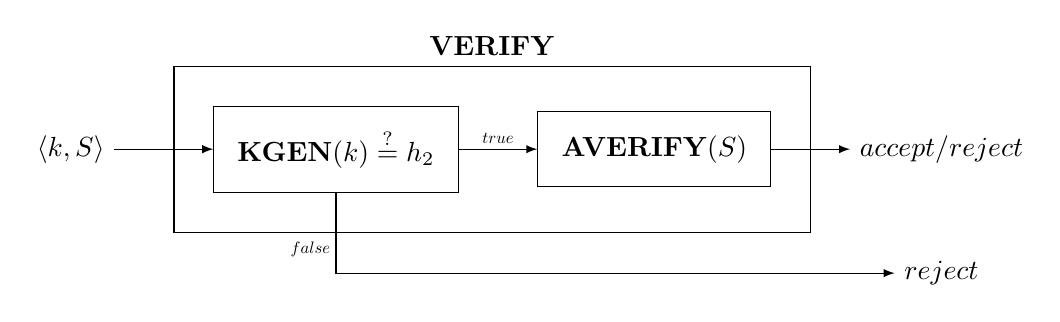
\begin{tikzpicture}[custom/.style = {rectangle, draw, align=center, inner xsep=3mm, inner ysep=3mm}, -latex]
				% nodes
				\node[custom] (kgen) {$\keygen(k) \overset{?}{=} h_2$};
				\node[custom, right=1cm of kgen.east] (averify) {$\averify(S)$};
				\node[fit={(kgen) (averify)}, draw, inner xsep=5mm, inner ysep=5mm, label={\verify}] (outer) {};
				
				\node[left=.75cm of outer.west] (input) {$\goedel{k,S}$};
				\node[right=1cm of averify.east] (output1) {$accept/reject$};
				\node[below=1cm of output1.south] (output2) {$reject$};

				% connections
				\draw (input.east) to (kgen.west);
				\draw (kgen.east) -- node[above, scale=0.6]{$true$} (averify.west);
				\draw (averify.east) to (output1.west);
				\draw  (kgen.south) |- node[left, scale=0.6, yshift=.5cm]{$false$} (output2.west);
			\end{tikzpicture}
		}
	\end{center}

	\textcolor{blue}{\small explain/show on sec. slides what $S$ contains}
\end{frame}


\begin{frame}
	\frametitle{Algorithm Synergy}

	\resizebox{.9\hsize}{!}{
		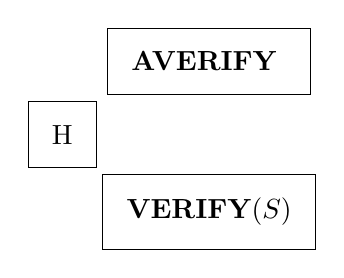
\begin{tikzpicture}[custom/.style = {rectangle, draw, align=center, inner xsep=3mm, inner ysep=3mm}, -latex]
			\node[custom] (asign) {\averify};
			\node[custom, below=1cm of asign] (verify) {$\verify(S)$};
			\node[custom, above left=.1cm of verify] (verify) {H};
		\end{tikzpicture}
	}

	\textcolor{blue}{TODO: add verification, signing, oracle/hash function synergy graph}

\end{frame}

  \subsection{Protocol}
  This section is responsible for providing an understanding of the concrete signature protocol and how the algorithms defined in \autoref{construction} should be used.

We will illustrate the protocol through an exemplary interaction between a party A(lice) and B(ob). 
The following description will be visually supported through \autoref{fig:concprotocol}. 

Firstly, we start by having both parties run the \textbf{SETUP} function to initialize all necessary variables for this scheme.
Our, so called, \textit{initial signer} continues with generating a keystone \(k\in\kspace\) alongside the corresponding keystone-fix \(f\in\kfspace\).
Keep in mind, that the keystone-fix is generated through \(\textbf{KGEN}(k)\).
We set, without loss of generality, Alice as our initial signer.
Continuing, the initial signer starts off by signing a message \(M_A\in\mespace\) through \textbf{ASIGN}, while providing the private keys of herself and Bob, her own private key \(x_A\) and the keystone-fix \(f\).
Afterwards, Alice sends the resulting ambiguous signature \(\sigma_A = \goedel{s_A, h_A, f}\) to Bob.
He verifies said signature by checking if \textbf{AVERIFY} returns \(accept\), for which he additionally provides their respective public keys, as well as, Alice's message \(M_A\).
Note, that we are not trying to encrypt or obfuscate the messages in any way.
Bob and Alice, repeat the signing and verification steps analogously for Bob with the \textit{same keystone-fix}, i.e. Bob generates and sends his ambiguous signature with \(f\) and Alice verifies it.
Lastly, if Alice is satisfied with Bobs signature, she publishes the keystone \(k\) with which both \textit{ambiguous signatures} will be binding for both parties.

The power of who is generating and holding the keystone-fix is the one thing that keeps the concurrent signature scheme to be \textit{truly fair}.
Because with this, the initial signer (i.e. the one that generates the keystone(-fix)) can withhold the keystone.
However, this would not be beneficial for the withholding party in real applications.
Moreover, even if the withholding party keeps the keystone, without releasing it, the other party is not bound to the signature, meaning it is at no disadvantage. 

\begin{figure}[htbp]
  \centering
  
  \resizebox{.99\hsize}{!}{
    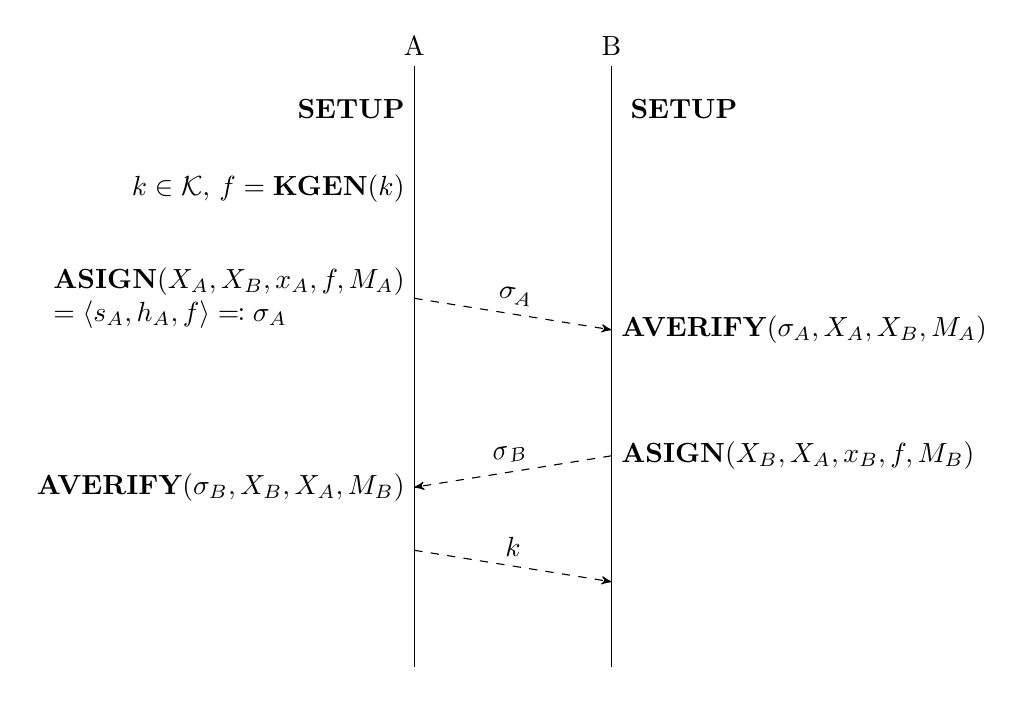
\begin{tikzpicture}[node distance=2cm,auto,>=stealth']
      \node[] (bob) {B};
      \node[left = of bob] (alice) {A};
      \node[below of=bob, node distance=8cm] (bobground) {};
      \node[below of=alice, node distance=8cm] (aliceground) {};
      
      % vertical lines
      \draw (alice) -- (aliceground);
      \draw (bob) -- (bobground);
    
      % setup
      \node[left, align=left] at ($(alice)!0.1!(aliceground)$) {\textbf{SETUP}};
      \node[right, align=right] at ($(bob)!0.1!(bobground)$) {~\textbf{SETUP}};
  
      % k keystone + KGEN
      \node[left, align=left] at ($(alice)!0.225!(aliceground)$) {$k\in\kspace$, $f = \textbf{KGEN}(k)$};
      
      % ASIGN + Arrow
      \node[left, align=left] at ($(alice)!0.4!(aliceground)$) {$\textbf{ASIGN}(X_A, X_B, x_A, f, M_A)$ \\ {$= \goedel{s_A, h_A, f} \eqqcolon \sigma_A$}};
      \draw[->, dashed] ($(alice)!0.4!(aliceground)$) -- node[sloped, above]{$\sigma_A$} ($(bob)!0.45!(bobground)$);
      
      % AVERIFY
      \node[right, align=center] at ($(bob)!0.45!(bobground)$) {$\textbf{AVERIFY}(\sigma_A, X_A, X_B, M_A)$};

      % ASIGN + Arrow
      \node[right, align=left] at ($(bob)!0.65!(bobground)$) {$\textbf{ASIGN}(X_B, X_A, x_B, f, M_B)$};
      \draw[->, dashed] ($(bob)!0.65!(bobground)$) -- node[sloped, above]{$\sigma_B$} ($(alice)!0.7!(aliceground)$);

      % AVERIFY
      \node[left, align=left] at ($(alice)!0.7!(aliceground)$) {$\textbf{AVERIFY}(\sigma_B, X_B, X_A, M_B)$};

      % keystone
      \draw[->, dashed] ($(alice)!0.8!(aliceground)$) -- node[above]{$k$} ($(bob)!0.85!(bobground)$);
    \end{tikzpicture}
  }

  \caption{Concurrent Signature Protocol - An Overview}
  \label{fig:concprotocol}
\end{figure}

% --------------------------------------------------------- Security Model
\section{Security Model}
\begin{frame}
	\frametitle{Concurrent Signature Protocol}

	\begin{itemize}
		\item Describing signature exchange between A(lice) and B(ob)
		\item Initial signer has to generate keystone
		\item Matching signer responds by using the same keystone-fix
		\item Alice and Bob both run \setup to set public variables
			\begin{itemize}
				\item A's and B's public- and private keys are $X_A$, $x_a$ and $X_B$, $x_B$, respectively
			\end{itemize}
	\end{itemize}
\end{frame}

\begin{frame}
	\frametitle{Concurrent Signature Protocol}

	\begin{enumerate}
		\item A picks a random keystone $k\in\kspace$ and computes $f = \textbf{KGEN}(k)$
		\item A computes ambiguous signature with $M_A \in \mespace$ being A's message 
			$$\sigma_A \coloneqq \goedel{s_A,h_A,h} = \asign(X_A, X_B, x_A, f, M_A)$$ 
		\item B verifies signature by checking
			$$\averify(\goedel{s_A, h_A, f}, X_A, X_B, M_A) = accept$$
			reject otherwise
		\setcounter{ResumeEnumerate}{\value{enumi}}
	\end{enumerate}
\end{frame}


\begin{frame}
	\frametitle{Concurrent Signature Protocol}

	\begin{enumerate}[start=\numexpr\value{ResumeEnumerate}+1]
		\item B picks message $M_B \in \mespace$ and creates own ambiguous signature
		$$\sigma_B \coloneqq \goedel{s_B,h_B,h} = \asign(X_B, X_B, x_A, f, M_B)$$
		\item A verifies this time with
			$$\averify(\goedel{s_B, h_B, f}, X_B, X_A, M_B) = accept$$
			with $f$ same keystone fix as before
		\item A sends keystone to B
	\end{enumerate}
\end{frame}

  \subsection{Fairness}
  \begin{frame}
	\frametitle{Fairness}

	\begin{itemize}
		\item \textbf{SETUP}, \textbf{KGen}, \textbf{KReveal}, \textbf{ASign} and \textbf{Private Key Extraction} Queries as in Ambiguity
		\item adversary $E$ outputs $S=\goedel{\underbrace{\goedel{s, h_1, f}}_{\eqqcolon\sigma},X_c, X_d, M}$
		\item Further $\averify(S)=accept$
		\item $E$ wins if one of the following holds
			\begin{itemize}
				\item $f$ was previous output from \keygen, no \textbf{KReveal} query was made and $\goedel{k, S}$ is accepted by \verify
				\item $E$ outputs $\goedel{\sigma',X_d, X_c, M'}$ with $\sigma' = \goedel{s', h_1', f}$ 
					\begin{itemize}
						\item $\averify(S') = accept$
						\item $\verify(\goedel{k,S}) = accept$
						\item $\verify(\goedel{k,S'}) = reject$
					\end{itemize}
			\end{itemize}
	\end{itemize}
\end{frame}

  \subsection{Ambiguity}
  \begin{frame}
	\frametitle{Ambiguity}

  	
  \begin{center}
    \resizebox{.95\hsize}{!}{
      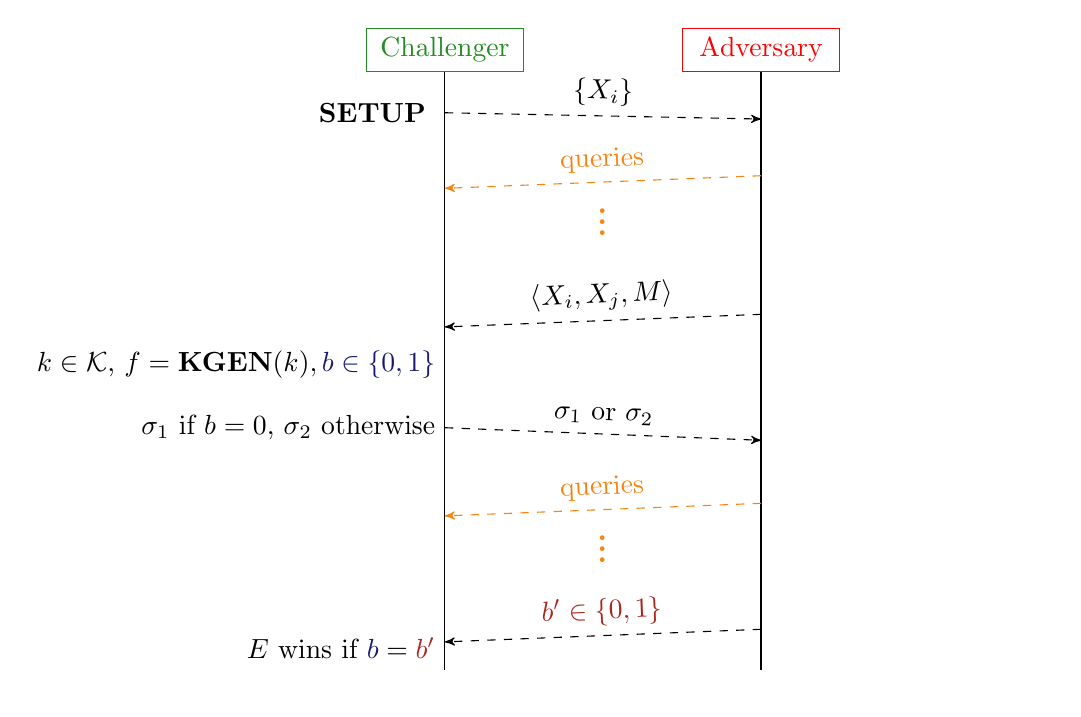
\begin{tikzpicture}[node distance=2cm,auto,>=stealth']
        \node[draw, minimum width = 2cm, color=Red] (adversary) {Adversary};
        \node[draw, minimum width = 2cm, color=ForestGreen, left = of adversary] (challenger) {Challenger};
        \node[below of=adversary, node distance=8cm] (adversaryground) {};
        \node[below of=challenger, node distance=8cm] (challengerground) {};
        
        % vertical lines
        \draw (challenger) -- (challengerground);
        \draw (adversary) -- (adversaryground);
      
        % setup
        \node[left, align=left] at ($(challenger)!0.1!(challengerground)$) {\setup};
        \visible<2->{\draw[->, dashed] ($(challenger)!0.1!(challengerground)$) -- node[sloped, above]{$\{X_i\}$} ($(adversary)!0.11!(adversaryground)$);}
        
        \visible<3->{\draw[->, dashed, BurntOrange] ($(adversary)!0.2!(adversaryground)$) -- node[sloped, above] (queries0) {queries} ($(challenger)!0.22!(challengerground)$);}
        \visible<3->{\node[below = 0mm of queries0, black] {\huge \textcolor{BurntOrange}{$\vdots$}};}

        \visible<4->{\draw[->, dashed] ($(adversary)!0.42!(adversaryground)$) -- node[sloped, above]{$\goedel{X_i, X_j, M}$} ($(challenger)!0.44!(challengerground)$);}

        \visible<5->{\node[left, align=left] at ($(challenger)!0.5!(challengerground)$) {$k\in\kspace$, $f = \textbf{KGEN}(k), \textcolor{MidnightBlue}{b\in\{0,1\}}$};}
        \visible<6->{\node[left, align=left] at ($(challenger)!0.6!(challengerground)$) {$\sigma_1$ if $b=0$, $\sigma_2$ otherwise};}

        \visible<7->{\draw[->, dashed] ($(challenger)!0.6!(challengerground)$) -- node[sloped, above]{$\sigma_1$ or $\sigma_2$} ($(adversary)!0.62!(adversaryground)$);}

        \visible<8->{\draw[->, dashed, BurntOrange] ($(adversary)!0.72!(adversaryground)$) -- node[sloped, above] (queries1) {queries} ($(challenger)!0.74!(challengerground)$);}
        \visible<8->{\node[below = 0mm of queries1, black] {\huge \textcolor{BurntOrange}{$\vdots$}};}

        \visible<9->{\draw[->, dashed] ($(adversary)!0.92!(adversaryground)$) -- node[sloped, above]{\textcolor{Mahogany}{$b'\in\{0,1\}$}} ($(challenger)!0.94!(challengerground)$);}
        
        \visible<10->{\node[left, align=left] at ($(challenger)!0.95!(challengerground)$) {$E$ wins if $\textcolor{MidnightBlue}{b}=\textcolor{Mahogany}{b'}$};}

        \node[right, align=center] at ($(adversary)!0.42!(adversaryground)$) {\phantom{{$k\in\kspace$, $f = \textbf{KGEN}(k)$}}};
      \end{tikzpicture}
    }
	\end{center}
\end{frame}

  \subsection{Unforgeability}
  \begin{frame}
	\frametitle{Unforgeability}

	\begin{itemize}[<+->]
		\item consider previous adversary-challenger game
		\item \textcolor{Red}{$E$} can query everything 
		\item eventually \textcolor{Red}{$E$} outputs tuple $S = (\sigma, X_c, X_d, M)$ 
		\item \textcolor{Red}{$E$} wins if $\averify(S) = accept$ and no Private Key Extraction Query was made and
      \begin{enumerate}
        \item No \asign query with our parameters, and no \textbf{Private Key Extraction} query for $X_c$ or $X_d$ 
	     	\item No \asign query with $\goedel{X_c, X_i, f, M}$, no \textbf{Private Key Extraction} query for $X_c$, and
		    	\begin{itemize}
            \item $f$ output from previous \keygen query or
            \item \textcolor{Red}{$E$} produces keystone $k$ such that $f = \keygen(k)$
          \end{itemize}
      \end{enumerate}
  \end{itemize}
\end{frame}

% --------------------------------------------------------- Proof of Lemmata
\section{Concrete Scheme}
\begin{frame}
	\frametitle{Concurrent Signature Protocol}

	\begin{itemize}
		\item Describing signature exchange between A(lice) and B(ob)
		\item Initial signer has to generate keystone
		\item Matching signer responds by using the same keystone-fix
		\item Alice and Bob both run \setup to set public variables
			\begin{itemize}
				\item A's and B's public- and private keys are $X_A$, $x_a$ and $X_B$, $x_B$, respectively
			\end{itemize}
	\end{itemize}
\end{frame}

\begin{frame}
	\frametitle{Concurrent Signature Protocol}

	\begin{enumerate}
		\item A picks a random keystone $k\in\kspace$ and computes $f = \textbf{KGEN}(k)$
		\item A computes ambiguous signature with $M_A \in \mespace$ being A's message 
			$$\sigma_A \coloneqq \goedel{s_A,h_A,h} = \asign(X_A, X_B, x_A, f, M_A)$$ 
		\item B verifies signature by checking
			$$\averify(\goedel{s_A, h_A, f}, X_A, X_B, M_A) = accept$$
			reject otherwise
		\setcounter{ResumeEnumerate}{\value{enumi}}
	\end{enumerate}
\end{frame}


\begin{frame}
	\frametitle{Concurrent Signature Protocol}

	\begin{enumerate}[start=\numexpr\value{ResumeEnumerate}+1]
		\item B picks message $M_B \in \mespace$ and creates own ambiguous signature
		$$\sigma_B \coloneqq \goedel{s_B,h_B,h} = \asign(X_B, X_B, x_A, f, M_B)$$
		\item A verifies this time with
			$$\averify(\goedel{s_B, h_B, f}, X_B, X_A, M_B) = accept$$
			with $f$ same keystone fix as before
		\item A sends keystone to B
	\end{enumerate}
\end{frame}

% Preliminaries
\begin{frame}
	\frametitle{Discrete Logarithmic Assumption}
\end{frame}
\begin{frame}
	\frametitle{Random Oracle}

	\begin{block}{Definition (Oracle)}
		An \textbf{oracle} (machine) is an abstract machine that takes an input and generates a solution for it without knowing its inner workings.
	\end{block}
	\begin{block}{Definition (Random Oracle)}
		A \textbf{random oracle} is a oracle, which fulfills the following properties
		\begin{itemize}
			\item returns each \textit{unique} request with a truly random value (chosen from output domain)
			\item repeated requests (always) return the same response
		\end{itemize}
	\end{block}
\end{frame}
\begin{frame}
	\frametitle{Definitions}

	\begin{definition}[SETUP]
		takes a security parameter $\ell$ as an input. Returns
		\begin{itemize}
			\item set of participants $\mathcal{U}$
			\item message space $\mathcal{M}$
			\item signature space $\mathcal{S}$
			\item keystone space $\mathcal{K}$
			\item keystone fix space $\mathcal{F}$
			\item function $KGEN: \mathcal{K} \to \mathcal{F}$
		\end{itemize}
	\end{definition}
\end{frame}

\begin{frame}
	\frametitle{Definitions}
	\begin{definition}[ASIGN]
	takes $\goedel{X_i, X_j, x_i, h_2,M}$
		\begin{itemize}
			\item $X_i$ and $X_j$ (with $X_i \neq X_j$) public keys
			\item $x_i$ private key
			\item 
		\end{itemize}
	\end{definition}
\end{frame}

\begin{frame}
	\frametitle{Definitions}
	\begin{definition}[AVERIFY]
	takes $\goedel{0}$
		\begin{itemize}
			\item 
		\end{itemize}
	\end{definition}
\end{frame}

\begin{frame}
	\frametitle{Definitions}
	\begin{definition}[VERIFY]
	takes $\goedel{0}$
		\begin{itemize}
			\item 
		\end{itemize}
	\end{definition}
\end{frame}
\begin{frame}
	\frametitle{Forking Lemma}
\end{frame}

\begin{frame}
	\frametitle{Unforgeability - Proof}
	
	\textit{Proof Idea:}
	\begin{enumerate}[<+->]
		\item Assumption: hardness of the discrete logarithm
		\item Proof by contraposition: Scheme is forgeable with an non-neglible probability
		\item Create system, that uses the adversary to solve the discrete logarithm problem
	\end{enumerate}
\end{frame}

\begin{frame}
	\frametitle{Proof - Setup}

	\begin{itemize}[<+->]
		\item need signature format $\goedel{r_1, h, r_2}$
		\begin{itemize}
			\item easily deriviable from $\sigma = \goedel{s, h_1, h_2}$
		\end{itemize}
		\item $H_1, H_2$ random oracles
		\item $E$ is forging-adversary
		\item $\mathcal{A}$ is an algorithm that solves the discrete logarithm problem
			\begin{itemize}
				\item simulates random oracles and challenger $C$
				\item input: $\goedel{g, X, p , q}$
				\item goal: find $x\in\ints_q$ s.t. $g^x = X \bmod p$
			\end{itemize}
	\end{itemize}
\end{frame}

\begin{frame}
	\frametitle{Proof - Simulation}

	\begin{center}
		\resizebox{\hsize}{!}{
			\begin{tikzpicture}[custom/.style = {rectangle, draw, align=center, minimum width=1.5cm, inner xsep=3mm, inner ysep=3mm}, -latex]
				% nodes
				\visible<3->{\node[custom] (adversary) {$E$};}
				\visible<4->{\node[above=.75cm of adversary] (adversary_input) {$\goedel{g, p, q}$};}
				\phantom{\node[below=.75cm of adversary, align=center] (forged_signature) {$\sigma = \goedel{s, h_1, f}$, \\ $X_c, X_d, M$};}

				\visible<5->{\node[custom, right=.75cm of adversary_input] (participants) {$\mathcal{U}$};}
				\visible<5->{\node[custom, right=.75cm of participants] (priv_keys) {$x_i$};}
				
				\visible<6->{\node[custom, right=.75cm of adversary] (pub_keys) {$X_i {\visible<7->{= g^{x_i} \bmod p}}$};}
				
				\visible<1->{\node[fit={(adversary_input) (priv_keys) (forged_signature)}, draw, outer ysep=2mm, inner xsep=5mm, inner ysep=5mm, label={\Large$\mathcal{A}$}] (outer_box) {};}
				\visible<2->{\node[left=.5cm of outer_box.west] (input) {$\goedel{g, X, p, q}$};}
				
				% connections
				\visible<2->{\draw (input.east) to (outer_box.west);}
				\visible<4->{\draw (adversary_input.south) to (adversary.north);}
				\visible<8->{\draw (pub_keys.west) to (adversary.east);}
				\phantom{\draw (adversary.south) to (forged_signature.north);}
			\end{tikzpicture}
		}
	\end{center}
\end{frame}

\begin{frame}
	\frametitle{Proof - Simulation}

	\begin{itemize}
		\item $H_1, H_2$\textbf{-Queries}
		\item \textbf{KGen-Queries}
		\item \textbf{KReveal-Queries}
		\item \textbf{ASign-Queries} 
		\item \textbf{Private Key Extraction-Queries}
	\end{itemize}
\end{frame}

\begin{frame}
	\frametitle{Proof - Simulation}

	\begin{center}
		\resizebox{\hsize}{!}{
			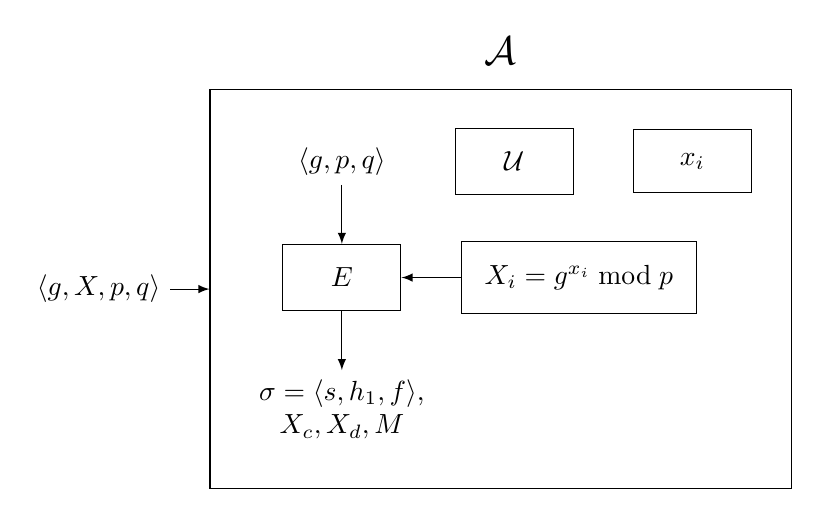
\begin{tikzpicture}[custom/.style = {rectangle, draw, align=center, minimum width=1.5cm, inner xsep=3mm, inner ysep=3mm}, -latex]
				% nodes
				\visible<1->{\node[custom] (adversary) {$E$};}
				\visible<1->{\node[above=.75cm of adversary] (adversary_input) {$\goedel{g, p, q}$};}
				\visible<2->{\node[below=.75cm of adversary, align=center] (forged_signature) {$\sigma = \goedel{s, h_1, f}$, \\ $X_c, X_d, M$};}

				\visible<1->{\node[custom, right=.75cm of adversary_input] (participants) {$\mathcal{U}$};}
				\visible<1->{\node[custom, right=.75cm of participants] (priv_keys) {$x_i$};}
				
				\visible<1->{\node[custom, right=.75cm of adversary] (pub_keys) {$X_i = g^{x_i} \bmod p$};}
				
				\visible<1->{\node[fit={(adversary_input) (priv_keys) (forged_signature)}, draw, outer ysep=2mm, inner xsep=5mm, inner ysep=5mm, label={\Large$\mathcal{A}$}] (outer_box) {};}
				\visible<1->{\node[left=.5cm of outer_box.west] (input) {$\goedel{g, X, p, q}$};}
				
				% connections
				\visible<1->{\draw (input.east) to (outer_box.west);}
				\visible<1->{\draw (adversary_input.south) to (adversary.north);}
				\visible<1->{\draw (pub_keys.west) to (adversary.east);}
				\visible<2->{\draw (adversary.south) to (forged_signature.north);}
			\end{tikzpicture}
		}
	\end{center}
\end{frame}

\begin{frame}
	\frametitle{Proof - Simulation}

	With valid signature, one of the following holds
	\begin{itemize}
		\item No \asign query with $\goedel{X_c, X_d, f, M}$, and no \textbf{Private Key Extraction} query for $X_c$ or $X_d$ 
		\item No \asign query with $\goedel{X_c, X_i, f, M}$, no \textbf{Private Key Extraction} query for $X_c$, and
			\begin{itemize}
				\item $f$ output from previous \keygen query or
				\item $E$ produces keystone $k$ such that $f = \keygen(k)$
			\end{itemize}
	\end{itemize}
\end{frame}

\begin{frame}
	\frametitle{Proof - Simulation}

	\begin{itemize}
		\item if $X_c \neq X_\alpha$, $\mathcal{A}$ aborts because it's lost
		\item Therefore assume: $X_c = X_\alpha = X$
		\item with second case we have:
			$$h = h_1 + f = H_2(g^s X_{c}^{h_1} X_d^f \bmod p ~\|~ M)$$
	\end{itemize}
\end{frame}

\begin{frame}
	\frametitle{Proof - Simulation}

	Case 1: $h = h_1 + f$ never appeared in previous signature query

	\begin{itemize}
		\item force $E$ to rerun simulation to produce $(r_1, h', r_2')$ with $h \neq h'$
	\end{itemize}

\end{frame}

% --------------------------------------------------------- Conclusion
\section{Conclusion}
\begin{frame}
	\frametitle{Conclusion}

  \begin{center}  
    \begin{itemize}
      \setlength\itemsep{1em}
      \item sign entities without a significant disadvantage
      \item ambiguous until all parties are committed
      \item still not \textcolor{Plum}{\textit{truly fair}}
    \end{itemize}
  \end{center}
\end{frame}

\end{document}